\chapter{Pruebas}
\label{chap:probas}

\lettrine{L}{as} pruebas de software constituyen un pilar fundamental para garantizar la calidad, la corrección y la estabilidad del sistema desarrollado. En este proyecto se ha adoptado un enfoque de pruebas automatizadas tanto para el backend como para el frontend, combinando distintos niveles de prueba según la naturaleza de cada subsistema. Para la aplicación Android, dadas las limitaciones de automatización en el entorno de desarrollo, se ha optado por un plan de pruebas manuales. Este capítulo describe la metodología empleada, las tecnologías utilizadas y el detalle de las pruebas realizadas en cada subsistema.

\section{Backend}

Las pruebas del backend se dividen en dos categorías: pruebas unitarias, que verifican la lógica de negocio de forma aislada mediante simulación de dependencias, y pruebas de integración, que comprueban el funcionamiento conjunto de los servicios con una base de datos real. Ambas están totalmente automatizadas y se ejecutan como parte del ciclo de compilación con Maven, lo que permite detectar problemas de regresión de forma temprana.

Tanto las pruebas unitarias como las de integración siguen una serie de convenciones. La nomenclatura de los métodos de prueba respeta el patrón \acrfull{tdd} con las claves \textit{given} (estado inicial), \textit{when} (acción que se prueba) y \textit{then} (resultado esperado). Además, se emplea el patrón \textit{Arrange-Act-Assert} para estructurar cada prueba de forma clara y legible, facilitando la comprensión de su propósito y lógica. 

\subsection{Pruebas unitarias}

Las pruebas unitarias se han implementado con JUnit 5 y Mockito. Este último permite simular los repositorios y dependencias externas de cada servicio, de modo que las pruebas se centran exclusivamente en la lógica de negocio sin involucrar la persistencia ni la base de datos. Esto permite validar casos límite, reglas de negocio y flujos de error de forma rápida y aislada, asegurando que cada unidad de código se comporta correctamente bajo diferentes escenarios. 

Para la creación de entidades de prueba se emplea el patrón \textit{Object Mother}, que proporciona fábricas estáticas con valores por defecto y métodos de personalización, facilitando la creación estándar y a la vez flexible de objetos sin saturar cada prueba con lógica de inicialización.

La siguiente imagen \ref{fig:object-mother} muestra un ejemplo de clase que sigue el patrón Object Mother para la entidad \texttt{Organization}, con métodos estáticos para generar instancias preconfiguradas y personalizables. Este patrón tiene numerosas ventajas como la reutilización de código, mantenibilidad y legibilidad alta y promueve la separación de la creación de datos para las pruebas con las pruebas en sí.

\begin{figure}[H]
  \centering
  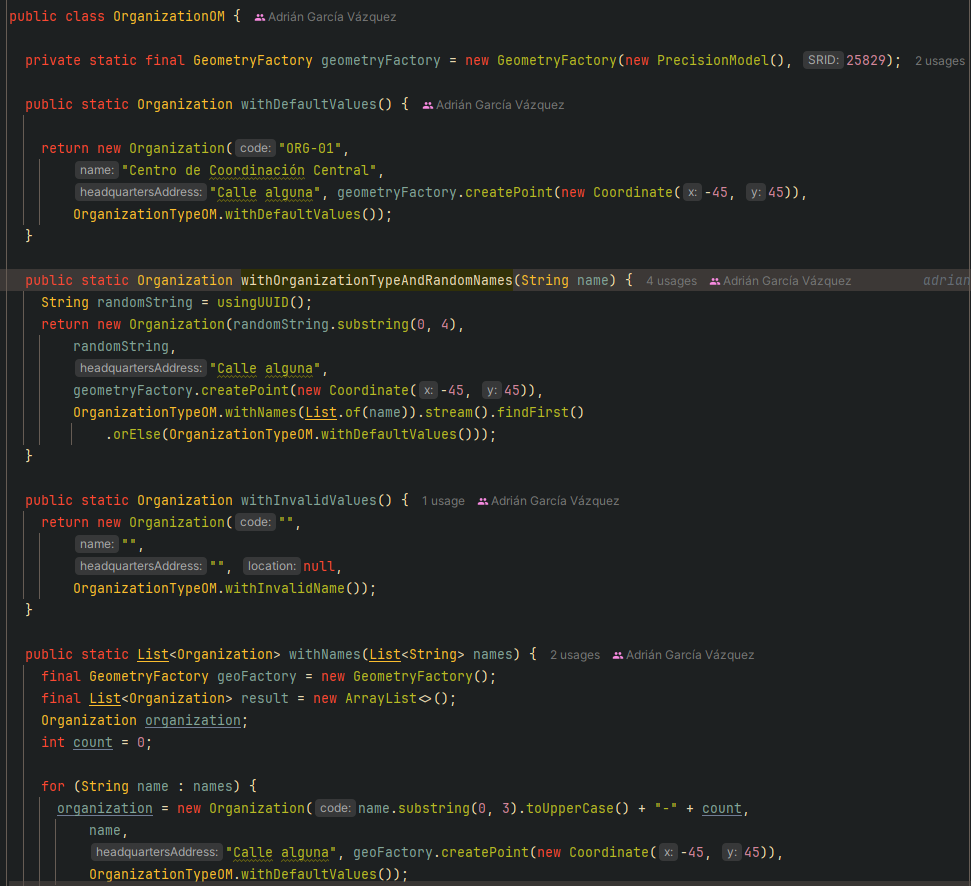
\includegraphics[width=\textwidth]{imaxes/organizacion-om.png}
  \caption{Código de una clase que sigue el patrón Object Mother}
  \label{fig:object-mother}
\end{figure}


\subsection{Pruebas de integración}

Las pruebas de integración utilizan Testcontainers con la imagen \textit{postgis/postgis}, que levanta una instancia efímera de PostgreSQL con PostGIS para cada ejecución. La base de datos se inicializa automáticamente con los mismos scripts SQL de creación de tablas, cuadrantes y datos de inicialización que se emplean en desarrollo (\texttt{01\_create\_tables.sql}, \texttt{02\_init\_quadrants.sql} y \texttt{03\_init\_data.sql}), lo que garantiza que el entorno de pruebas es representativo del real. Todas las pruebas de integración extienden la clase base abstracta \texttt{IntegrationTest}, que configura \texttt{@SpringBootTest}, \texttt{@Transactional} y la inyección automática de propiedades de conexión al contenedor PostgreSQL.

Esta configuración de las pruebas de integración permite validar la lógica de negocio en un entorno realista, con una base de datos real y sin simulaciones. Se han diseñado pruebas para cubrir tanto los flujos normales como los casos de error, incluyendo validaciones de negocio, manejo de excepciones y casos límite. 


\subsection{Cobertura de las pruebas}

En esta imagen \ref{fig:coverage} se muestra la cobertura de las pruebas unitarias e integración del backend. La cobertura es un indicador que aporta confianza pero no garantiza la ausencia de errores, por lo que se ha complementado con un análisis de casos límite y validaciones de negocio en las pruebas de integración. Se ha tratado de alcanzar una cobertura elevada en la capa de servicios mediante una batería de tests de integración que validan tanto los flujos normales como los casos de error, asegurando que la lógica de negocio se comporta correctamente en un entorno realista con una base de datos real. 

\begin{figure}[H]
  \centering
  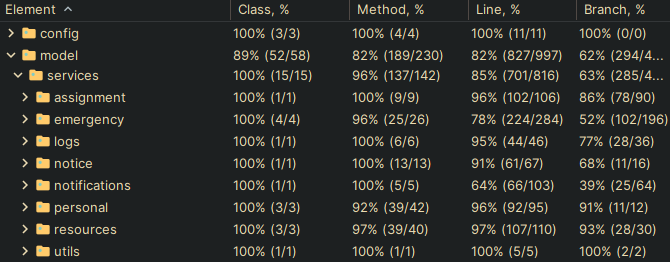
\includegraphics[width=\textwidth]{imaxes/coverage.png}
  \caption{Cobertura de las pruebas del backend}
  \label{fig:coverage}
\end{figure}

\section{Frontend}

Para el frontend se ha adoptado una estrategia de pruebas automatizadas centrada en dos niveles: la lógica pura de la aplicación (funciones de validación, transformación de coordenadas y reductores de estado) y el renderizado de componentes clave. 

Las pruebas se han implementado con Vitest, el ejecutor de tests nativo de Vite. Para el renderizado de componentes se ha empleado React Testing Library, que fomenta pruebas centradas en el comportamiento observable desde la perspectiva del usuario en lugar de detalles de implementación interna.

Se han creado tests distribuidos en las siguientes categorías:

\begin{itemize}
  \item \textbf{Lógica pura:} funciones de validación de formularios (email, teléfono, DNI), formateo de fechas y transformación de coordenadas geográficas a UTM (y viceversa). Estos tests verifican la corrección de la lógica de negocio en el frontend sin necesidad de montar componentes ni depender del navegador, lo que los hace extremadamente rápidos y fiables.
  \item \textbf{Reductores de estado:} pruebas sobre los slices de Redux (\texttt{LoginSlice}, \texttt{themeSlice}) que validan el estado inicial, las transiciones de estado y los selectores.
  \item \textbf{Componentes de interfaz:} renderizado de componentes clave como \texttt{EmergencyTypeIcon} (mapeo de nombres de emergencia a iconos), \texttt{BackButton}, \texttt{NotFoundPage} y \texttt{TeamNotFoundPage}. Estos tests verifican que los componentes se renderizan sin errores, que muestran los elementos esperados (iconos, enlaces, imágenes) y que responden correctamente a las propiedades recibidas.
\end{itemize}

La siguiente imagen \ref{fig:vitest} muestra la ejecución completa de los tests del frontend con Vitest:

\begin{figure}[H]
  \centering
  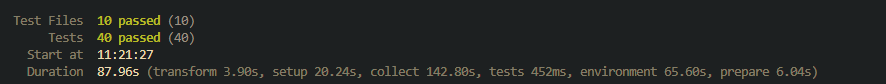
\includegraphics[width=\textwidth]{imaxes/vitest.png}
  \caption{Ejecución de los tests del frontend con Vitest}
  \label{fig:vitest}
\end{figure}

Esta batería de tests automatizados aporta tres beneficios principales. En primer lugar, permite detectar de forma temprana regresiones en la lógica de validación y formateo, que son propensas a errores silenciosos. En segundo lugar, garantiza que los componentes críticos se renderizan correctamente tras cambios en las dependencias o en la estructura del código. Por último, al ejecutarse con Vitest, se integran en el flujo de desarrollo con una ejecución rápida que no interrumpe el trabajo del desarrollador.

Además de las pruebas automatizadas, se ha complementado la validación con un plan de pruebas manuales exhaustivas de la interfaz, que permiten validar la experiencia de usuario, la usabilidad y el comportamiento visual en diferentes dispositivos y navegadores. Dado que el frontend presenta una interfaz gráfica compleja con mapas interactivos y componentes dinámicos, las pruebas manuales cubren aspectos que las pruebas automatizadas no alcanzan, como la correcta visualización del mapa, la respuesta a eventos de usuario y la navegación entre pantallas.

\section{Aplicación Android}

